\documentclass[10pt,a4paper]{cerndoc}

\CernDocSection{CERN BE-CO-HT}
\CernDocBorderColor{150,0,0}

\CernDocType{Technical Specifications}
\CernDocTitle{Gennum GN4124 Core For FMC Projects}
\CernDocEditedBy{Simon Deprez}
\CernDocCheckedBy{}
\CernDocDate{July 2010}
\CernDocAbstract{This technical specification describes the HDL controller for Gennum GN4124 chip. It provides a Wishbone master for control and status registers access and a DMA controller for high speed data transfers.}

\begin{document}
  \cerntitle
  \section*{Revision History}
  \begin{tabularx}{\textwidth}{|p{3cm}|p{3cm}|X|}
    \hline \textbf{Version}&\textbf{Date}&\textbf{Notes}\\ \hline \hline
    0.1 & 10-06-2010 & Initial release\\ \hline
    0.2 & 12-07-2010 & First draft\\ \hline

  \end{tabularx}

  \tableofcontents
  \listoffigures
  \clearpage

  \section*{Introduction}
  \addcontentsline{toc}{section}{Introduction}
This specification describes how the core work internally. For each internal block, we give a summary description of its function.
The figure \ref{fig:GN4124core_arch} show the core with all main blocks.

The structure of this cores and some signals names are based on Gennum cores \emph{Lambo} and \emph{Lotus}. 

\begin{figure}[!ht]
  \centering
    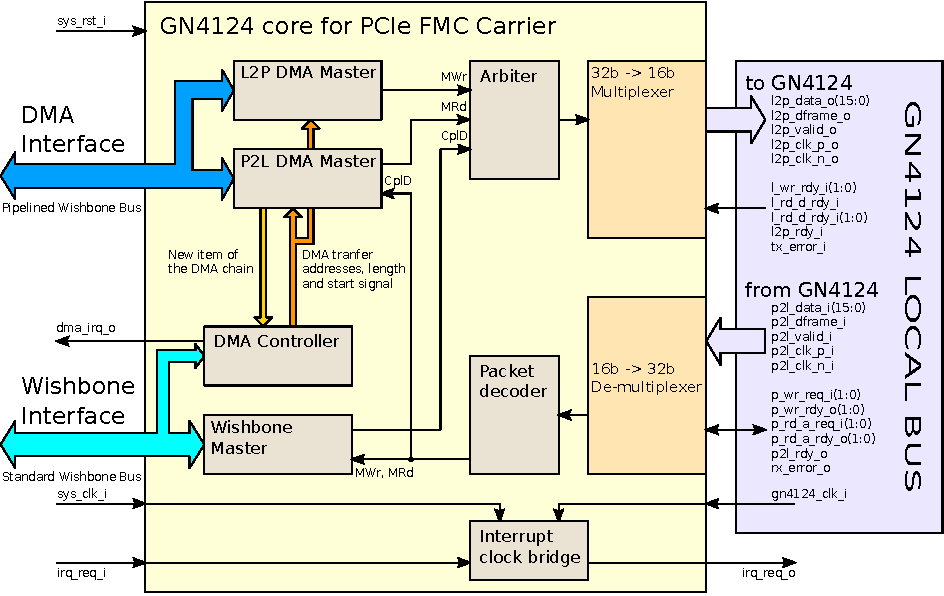
\includegraphics[width=\textwidth]{GN4124core_arch.pdf}
  \caption{GN4124 core for PCIe FMC carrier}
  \label{fig:GN4124core_arch}
\end{figure}

  \section{De-multiplexer}
  This block takes the double data rate 16-bit P2L (PCI Express to Local Bus direction) bus from the GN4124 device and converts it to a single data rate 32-bit bus for use inside the GN4124 core.
  
  \section{Multiplexer}
  It takes the internal single data rate 32 bit data and transmits it as double data rate 16-bit data on the L2P (Local Bus to PCI Express direction) bus.
  
  \section{Packet decoder}
    This block extracts header information, address, data, byte enables, and timing controls of the packets from the GN4124 chip. It provides signals like :
\begin{packed_item}
  \item Type of packet (target read request, target write request, master read completion \dots) 
  \item Begin of packet  
  \item Address that will increment with data
  \item Data
  \item End of packet   
\end{packed_item}

\section{Wishbone master}
  The Wishbone master implements a master for the Wishbone interconnection bus. It transforms a PCIe write into a Wishbone write and a PCIe read into a Wishbone read. Only single word reads and writes are supported. PCI express burst are divided in sigle reads and writes.
  
  Data are coming from the packet decoder. Wishbone signals are generated and the master waits for an acknowledge. The incoming requests are saved in a FIFO. The FIFO depth is 16. The Wishbone master is allowing the GN4124 chip to send a request only if the FIFO is empty. The latency of the transfer between the GN4124 chip and the Wishbone master makes this FIFO necessary.



\section{DMA controller}
  
\begin{figure}[!ht]
  \centering
  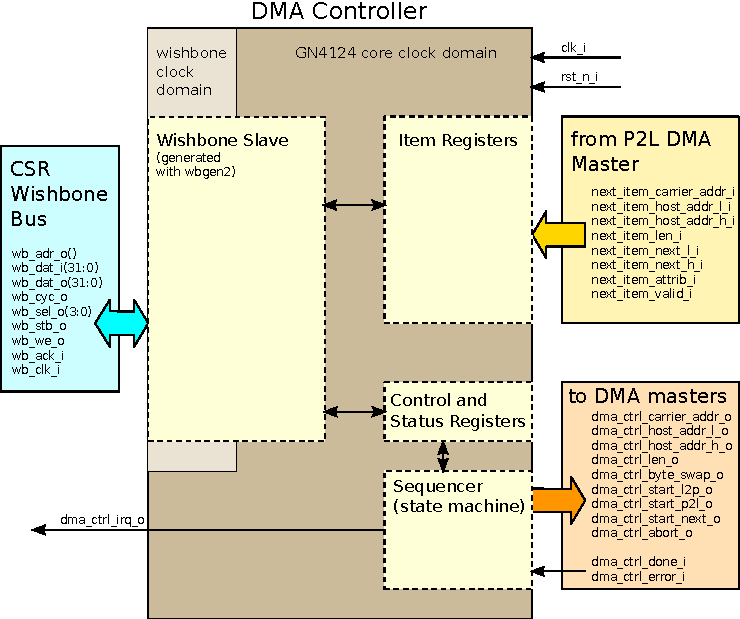
\includegraphics[width=\textwidth]{GN4124core_DMA_controller.pdf}
  \caption{DMA controller}
  \label{fig:GN4124core_dma_ctrl}
\end{figure}
  
The DMA controller is a Wishbone slave controlled from the PCI Express host with the Wishbone master (see the functional specification). The figure \ref{fig:GN4124core_dma_ctrl} shows the internal of the DMA controller.

The transfer starts when the first bit (LSB) of the DMACTRLR register is asserted. One of the two signals, \verb+dma_ctrl_start_L2P_o+ and \verb+dma_ctrl_start_P2L_o+, is set to '1' for one clock cycle. The \verb+dma_ctrl_start_L2P_o+ signal controls the DMA L2P master that performs transfers from the carrier to the PCI Express host and the \verb+dma_ctrl_start_P2L_o+ signal controls the DMA P2L master that performs transfers from the PCI Express host to the carrier.

The DMA controller waits for the \verb+dma_ctrl_done_i+ signal from one of the two DMA masters that indicates the end of the transfer. The \verb+dma_ctrl_error_i+ signal indicates the end of the transfer if an error occurs.

After the end of a transfer, if this transfer is not the last, the controller ask to the P2L DMA master the new item of the DMA chain. The \verb+next_item_valid_i+ signal indicates that the DMA master can read the new DMA chain item from the P2L DMA master and starts the new cycle


\begin{figure}[!ht]
	\centering
		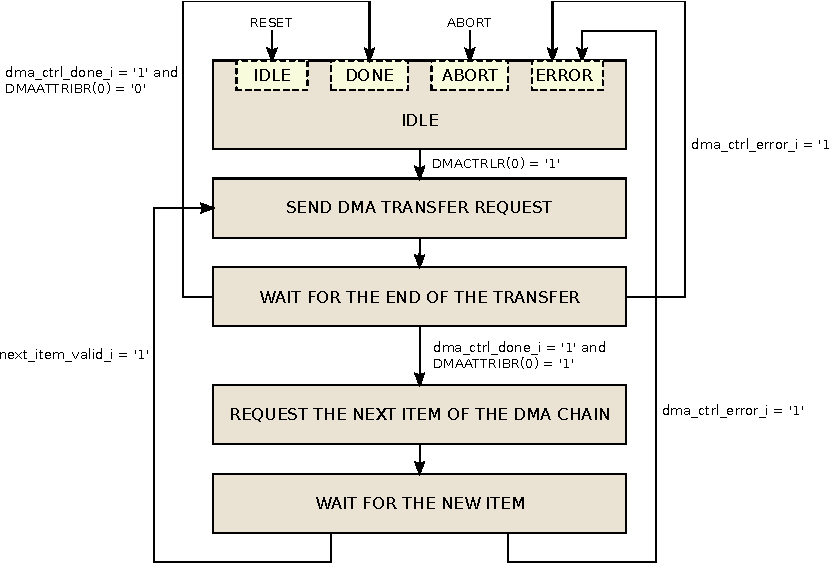
\includegraphics[width=\textwidth]{State_Machine_DMA_controller.pdf}
	\caption{DMA controller state machine}
	\label{fig:GN4124core_dma_ctrl_state_machine}
\end{figure}

  \section{L2P DMA Master}
The L2P DMA master performs data transfers from the PCI Express host to the FMC carrier. The transfer is split in small blocks of data. The length of this blocks can be configured.

The L2P DMA master sends a master read request on the DMA interface and waits for answer. This transfer is clocked by the \verb+sys_clk_i+ signal. The received data are stocked in a FIFO. 

When a block of data is in the FIFO, the DMA master sends a master write request to the PCI Express host. This operation is clocked by the GN4124 Local Bus Clock.
  

\begin{figure}[!ht]
	\centering
		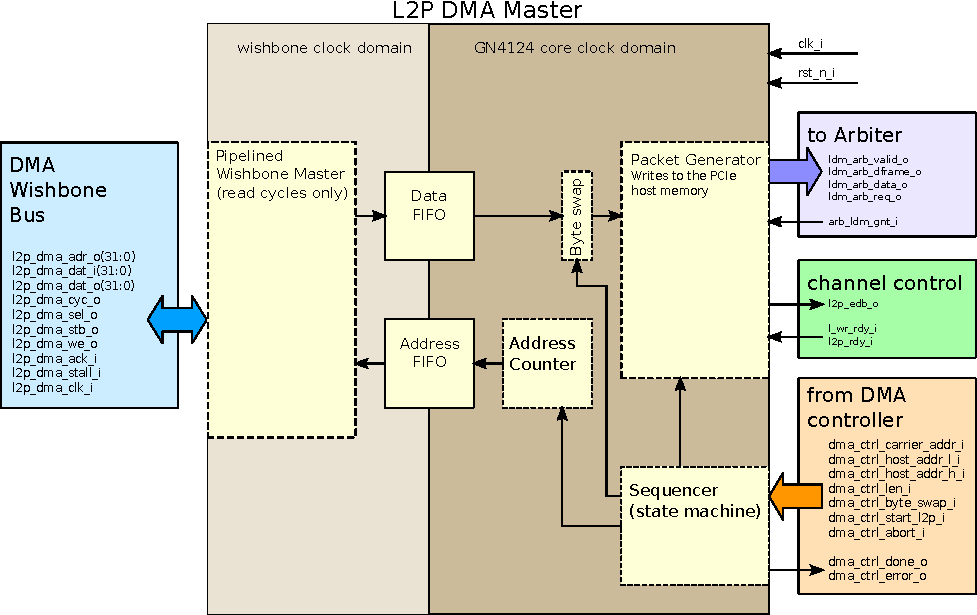
\includegraphics[width=\textwidth]{GN4124core_L2P_DMA_master.pdf}
	\caption{L2P DMA master}
	\label{fig:GN4124core_l2p_dma_master}
\end{figure}


 \section{P2L DMA Master}
 
 The P2L DMA master performs data transfers from the FMC carrier to the memory of the PCI Express host. The transfer is split in small blocks of data. The length of this blocks can be configured.
 
 The P2L DMA master sends a memory read request toward the GN4124 chip and waits for the answer. This operation is clocked by the GN4124 Local Bus Clock. The received data are stocked in a FIFO. 
 
When a block of data is in the FIFO, the DMA master starts a master write cycle on the DMA interface of this block. This transfer is clocked by the \verb+sys_clk_i+ signal. 
 
 \begin{figure}[!ht]
	\centering
		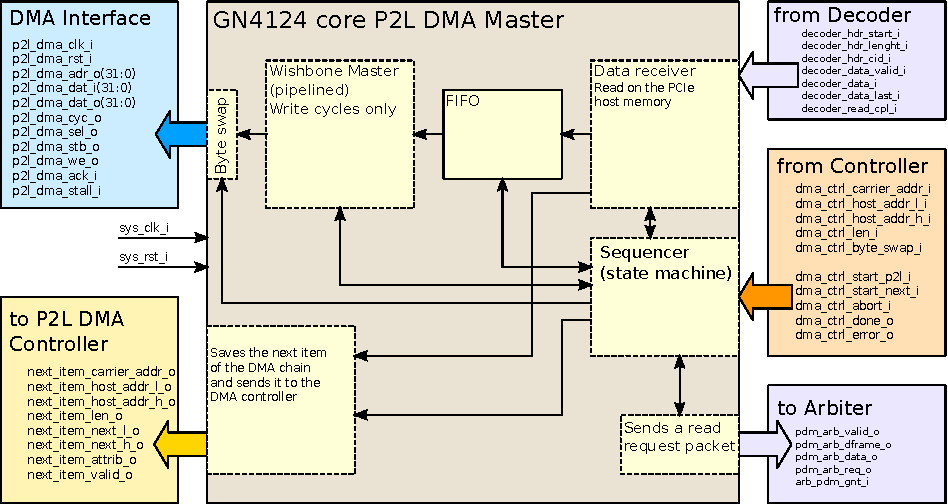
\includegraphics[width=\textwidth]{GN4124core_P2L_DMA_master.pdf}
	\caption{L2P DMA master}
	\label{fig:GN4124core_p2l_dma_master}
\end{figure}
 
 \section{Arbiter}
Arbitrate between Wishbone master and the two DMA masters. The arbiter is waiting for a request signal from one of this blocks and it grants the bus to the first requester until the end of the packet.

The highest priority is for Wishbone master.
 
  \section{Interrupt clock bridge}
  It transforms input interrupt one-tick-long pulse clocked by \verb+sys_clk_i+ in a one-tick-long pulse clocked by the GN4124 local bus clock.
\end{document}



